% !TEX root = ../thesis.tex

\chapter{绪论}

\section{基于深度学习的计算机视觉技术} \label{intro_dl}
以深度学习为代表的机器学习算法近年来在学术研究与生产应用的各个领域中备受关注。凭借其较强的特征与知识表征能力,飞速发展的深度学习算法逐渐在计算机视觉,自然语言处理,语音识别等识别与感知挑战中取得接近甚至超越人类的表现。%(加Cite呀)
深度学习模型往往依赖大规模数据集通过反向传播算法训练、优化得到的模型的权重参数,输入数据与这些权重参数进行的运算最终输出各类检测或识别的推理结果。无论是前向推理还是反向传播训练都需要处理存在大量的矩阵计算,因而深度学习的发展也离不开相关系统框架以及硬件架构的针对性优化与发展。\par
深度学习算法源于多层感知机模型(MLP)的不断改进与优化。MLP是一由全连接层(权重矩阵)和非线性激活函数共同构成的浅层神经网络。随着相关理论以及计算机算力的发展,神经网络的层数逐渐变深,不同类型的网络连接层、网络结构相继被提出。这一系列的发展使得深度学习模型有了更强的信息提取能力,在性能上逐步超越传统的人工设计的专家系统。\par
在计算机视觉领域,深度学习模型主要以卷积神经网络(CNN)的形式的存在。CNN借鉴了传统数字图像处理中卷积操作的概念,它权重共享以及平移不变的特性一方面大大减少了深层神经网络的参数,另一方面体现了CNN算法对不同图像特征提取的普遍适应性。
% emmm 要不要加个公式意思一下呢。。。 算了。。。
LeNet是CNN的早期代表模型,它被成功应用到了手写数字识别任务上。2012年的AlexNet使用了在GPU上实现的深层卷积神经网络结构,在当年的大规模视觉识别挑战(ImageNet)中取得了突破性的精度提升。AlexNet的出色表现也直接催生了后续深度学习技术的井喷式发展,从VGG,Inception,到ResNet,再到如今的网络架构搜索(NAS),CNN模型在精度和性能上都在不断地提升。如今各类视觉任务往往会利用这些出色的网络架构作为骨架来提取图像中的特征知识。\par
在具体视觉应用领域,计算机视觉也在近年来做到了从最初图像分类,人脸识别到目标检测,关键点检测,图像分割,图像生成等应用的全面发展。以目标检测为例,最开始R-CNN提出了区域推荐(Region Proposal)的方式完成目标检测。后来又有如Fast R-CNN,Faster R-CNN,Mask RCNN等算法将以区域推荐为主的检测方式逐步优化,不断提高模型的精度与运行效率。同时也有以YOLO系列为代表一系列检测算法通过对检测任务直接进行端对端的神经网络训练,模型的精简使得这种方法可以实现目标检测的实时推理。这些日益成熟的深度学习计算机视觉视觉也为无人驾驶,智能机器人,智慧城市等新兴研究方向提供了必要的技术支持,会在以后的生产生活中发挥更重要的作用。\par
如今深度学习算法在各个领域中已取得了初步的成效,当前深度学习技术发展主要关注在模型的压缩、剪枝、量化方法,自动化的机器学习算法开发(AutoML),深度神经网络黑盒模型的可解释性与安全性分析等方面,以提高深度学习模型的计算性能,开发效率以及应用可靠性。

\section{视频流处理模型与流程}\label{intro_vp}
从广义上来讲,视频流处理是对视频流信息进行一系列的数字信号处理以满足特定应用场景对视频资源的需求。传统意义上的视频处理任务包括视频压缩与编码,视频超分辨,视频插帧,视频内容分析等多个方面。数字图像处理技术的长期发展已经使一些传统视频处理任务有如编码、压缩、降噪、防抖等有了较好的解决方案。因此本文讨论的视频流处理主要是指对视频流内容的分析与检测,而这类视频分析任务如今的发展也是与\ref{intro_dl}中讨论的基于深度学习的计算机视觉算法有着密切的关系。\par
对视频分析任务我们又可以细分为目标检测与追踪,动作感应,姿态识别,图像分割,图像/视频增强等具体的应用类型。% 讲一下这些复杂CNN模型吧
这些在视频理解任务中使用到的深度学习视觉算法往往会由多个神经网络模型进行组合而成。首先,预处理后数据会在经过一些利用大型数据集预训练的经典CNN网络(如VGG, ResNet, MobileNet等)从原始输入图片中提取出高维特征信息。然后再将利用这些特征信息作为特定任务的神经网络的输入进行接下来机器学习分类或回归任务。这种算法模式常见于目标检测,图像分割,以及图像增强等任务中,代表模型有R-CNN系列,DeepLab系列,以及其他解码-编码(Encoder-Decoder)模式的图像生成模型。另一种常见的应景场景是更直接的多模型多步骤应用,比如在一些如人脸,人体的关键点检测上。为了保证模型的精度,这类任务往往需要先来运行一个相关目标检测的神经网络来获得目标的检测边框,利用获得的检测边框对原始图片输出进行进行再次的剪裁、缩放、旋转等操作,然后将处理得到的图片送入关键点检测的回归预测模型中,最终
获得检测结果。% e.g. alpha pose, MTCNN
除此之外,更为综合的视频分析可能需要对同一视频源进行多类型的视频识别任务,检测与理解。如CMU的开源项目OpenPose,有三个相对独立的神经网络算法分支同时对视频中的人体骨架,手部姿态以及人脸关键点进行检测与估计。\par
\begin{figure}[!htp]
    \centering
    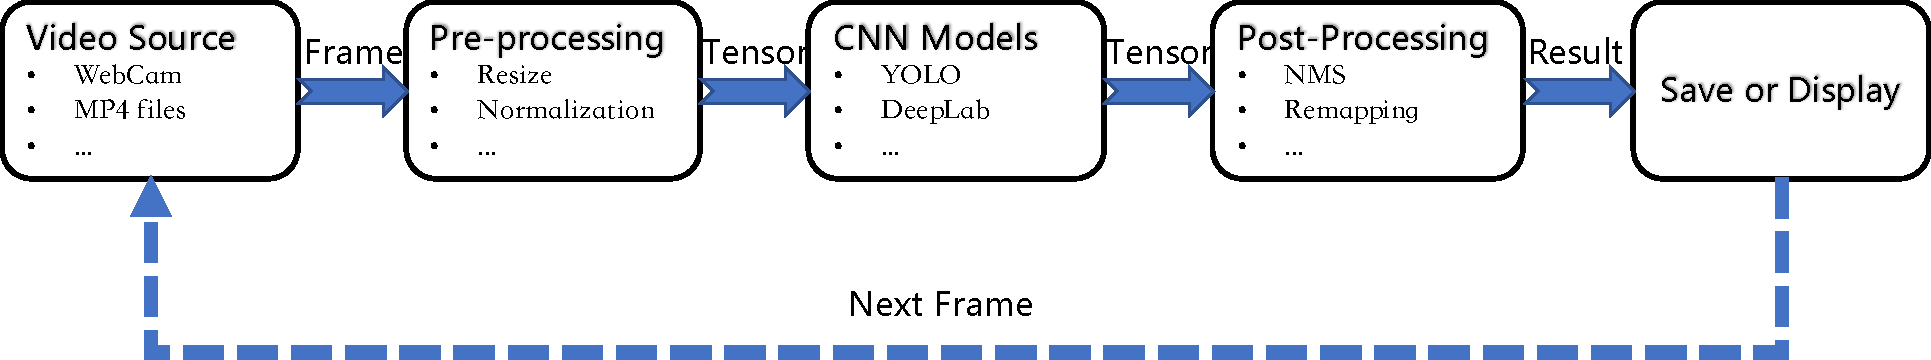
\includegraphics[width=\textwidth]{figure/video_proc_flow.pdf}
    \caption{深度学习下视频流处理的一般流程}
    \label{fig:video_proc_flow}
\end{figure}
在深度学习技术的背景下,虽然这些视频分析任务会使用到不同的机器学习算法的组合,但是也存在着许多共通的处理流程。% (emmm,可以考虑加一个流程示意图)
一般情况下,视频流的处理可以看作是在连续的视频帧上做图像的视觉计算。因此,视频处理通常由视频流的读取,视频帧的预处理,视觉算法模型(CNN)的运行,算法推理结果的后处理,以及结果的输出与展示这几部分共同来构成,如图\ref{fig:video_proc_flow}所示。本文接下来要讨论的视频流处理的优化工作也是基于对视频处理的这种理解与抽象。\par

\section{视频流处理的优化策略}
在\ref{intro_vp}中讨论的视频流处理过程可以进行多层面的优化。从底层硬件到系统运行框架再到算法层面,都有着相应的优化工作。一些相关优化工作也会在\ref{related_work}部分做进一步的介绍。
\section{论文的主要内容与章节安排}





